\documentclass{standalone}
\usepackage{pgfplots}
\pgfplotsset{
  compat=1.18, 
  trig format=rad, 
  ticklabel style = {font=\footnotesize},
  axis equal image,
}

\begin{document}
  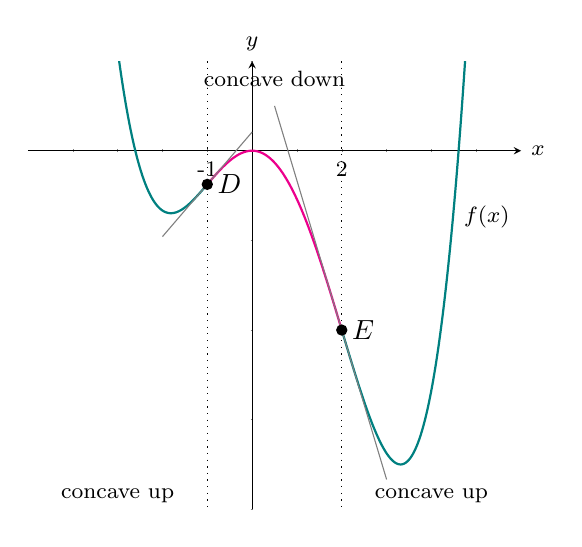
\begin{tikzpicture}
    \begin{axis}[
      axis lines=middle,
      % width=5in, height=5in,
      ymin=-8, ymax=2,
      xmin=-5, xmax=6,
      % ymin=-4, ymax=4,
      xlabel={\footnotesize \(x\)},
      xlabel style={at={(ticklabel* cs:1)}, anchor=west},
      ylabel={\footnotesize \(y\)},
      ylabel style={at={(ticklabel* cs:1)}, anchor=south},
      axis line style = {very thin},
      % xticklabels={,,},
      yticklabels={,,},
      xtick={-4,-3,-2,-1,0,1,2,3,4,5},
      xticklabels={,,,-1,,,2,},
      samples=500,
      % grid=both,
      % grid style={line width=.2pt, draw=gray!20},
      % minor tick num=1, 
      smooth,
      thick,
      no markers,
      tickwidth={1pt},
      ]
      % sage: f(x) = ((x+1)*(x-2)).integrate(x).integrate(x)
      \addplot[no markers, smooth, teal, domain=-4:-1] {1/12*x^4 - 1/6*x^3 - x^2};
      \addplot[no markers, smooth, magenta, domain=-1:2] {1/12*x^4 - 1/6*x^3 - x^2};
      \addplot[no markers, smooth, teal, domain=2:6] {1/12*x^4 - 1/6*x^3 - x^2};
      \addplot[thin, gray, domain=0.5:3] {8/3 - 10*x/3};
      \addplot[thin, gray, domain=-2:0] {7*x/6 + 5/12};
      % \node[above] at (0,0) {\footnotesize \(-x^{2}\) is concave down};
      \filldraw (-1,-3/4) circle (0.1) node[right] {\(D\)};
      \filldraw (2,-4) circle (0.1) node[right] {\(E\)};
      \addplot[thin, dotted] coordinates { (-1, 10) (-1, -10) };
      \addplot[thin, dotted] coordinates { (2, 10) (2, -10) };
      \node at (-3, -7.7) {\footnotesize concave up};
      \node[above] at (0.5, 1.2) {\footnotesize concave down};
      \node at (4, -7.7) {\footnotesize concave up};

      \node[below right] at (4.5,-1) {\footnotesize \(f(x)\)};
    \end{axis}
  \end{tikzpicture}
\end{document}
